\name{Diego Barquero Morera}
\address{Address : Italy, Trento, Via della Malpensada 140}
\address{Mobile (Costa Rica) : (+506) 8714 4835, Mobile (Italy) : (+39) 371 5704162}
\address{Email : \href{mailto:diego.barqueromorera@studenti.unitn.it}{diego.barqueromorera@studenti.unitn.it} $\qquad$ \href{https://github.com/DiegoBarMor}{GitHub} $\qquad$ \href{https://www.linkedin.com/in/diego-barquero-morera-98863020b/}{LinkedIn}}
\begin{document}


%\scriptsize{\small}
%--------------------------------------------------------------------
%    EDUCATION SECTION
%--------------------------------------------------------------------

\begin{rSection}{Education}

    % \vspace{\baselineskip}
    %
    % \begin{rSubsection}{\small{Physical characterization of protein/ligands binding sites for augmented reality visualization} \\ Université Paris Cité}{01.03.2023–31.10.2023}{Internship}{Paris, Île-de-France, France}
    %     \item[] Develop modules for a computer interface to interactively docking small ligands to proteins. The development involves both physical modelling of the interaction of the systems and writing the code for the modules for the visualization software UnityMol.
    % \end{rSubsection}

    \vspace{\baselineskip}

    {\bf \href{https://u-paris.fr/en/}{Université Paris Cité (UPC), Paris, France}} \hfill {01.03.2023–31.10.2023} \\
    \textit{Internship}\\
    Internship title: "Physical characterization of protein/ligands binding sites for augmented reality visualization"\\

    {\bf \href{https://www.unitn.it/}{Università degli Studi di Trento (Unitn), Trento, Italy}} \hfill {13.09.2021-14.12.2023} \\
    \textit{Master of Science in Quantitative and Computational Biology}\\
    Thesis title: "Physical characterization of protein and RNA binding sites and their graphical representation in the molecular visualization software UnityMol"\\

    {\bf \href{https://www.tum.de/en/}{Technical University of Munich (TUM), Munich, Germany}}\hfill {01.04.2019-30.09.2019}\\
    \textit{Exchange Program}\\
    Attended courses in the Faculty of Chemistry (Molecular Biology and Organic Chemistry)\\

    {\bf \href{https://www.tec.ac.cr/}{Costa Rica Institute of Technology (TEC), Cartago, Costa Rica}} \hfill {08.02.2016-02.09.2021} \\
    \textit{B.Sc. in Biotechnology Engineering}\\
    Thesis title: "Proposal of metabolic flux comparison by adapting algorithms for metabolic pathways"\\
    Grade: 100/100 with distinction


\end{rSection}
%--------------------------------------------------------------------
%    TECHNICAL STRENGTHS SECTION
%--------------------------------------------------------------------

\begin{rSection}{Competences}
    \vspace{\baselineskip}
    \subsection*{}

    %%%%%%%%%%%%%%%%%%%%%%%%%%%%%%%%%%%%%%%%%%%%%%%%%%%%%%%%%%%%%%%%%%%%%%%%%%%%%%
    \begin{table}[h!]
        \centering
        \captionof*{table}{Computer Languages}
        \begin{tabular}{llll}
            %%%%%%%%%%%%%%%%%%%%%%%%%%%%%%%%%%%%
            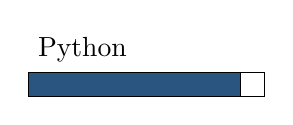
\begin{tikzpicture}
                \node [anchor=west] at (0,.6) {Python};
                \draw [fill=white] (0,0) rectangle (3,.3);
                \draw [fill={rgb:red,1;green,2;blue,3}] (0,0) rectangle (2.7,.3); %90%
            \end{tikzpicture} &

            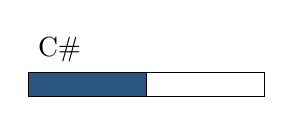
\begin{tikzpicture}
                \node [anchor=west] at (0,.6) {C\#};
                \draw [fill=white] (0,0) rectangle (3,.3);
                \draw [fill={rgb:red,1;green,2;blue,3}] (0,0) rectangle (1.5,.3); %50%
            \end{tikzpicture} &

            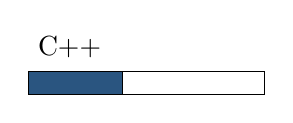
\begin{tikzpicture}
                \node [anchor=west] at (0,.6) {C++};
                \draw [fill=white] (0,0) rectangle (3,.3);
                \draw [fill={rgb:red,1;green,2;blue,3}] (0,0) rectangle (1.2,.3); %40%
            \end{tikzpicture} &

            
\begin{tikzpicture}
                \node [anchor=west] at (0,.6) {JavaScript, Java};
                \draw [fill=white] (0,0) rectangle (3,.3);
                \draw [fill={rgb:red,1;green,2;blue,3}] (0,0) rectangle (0.75,.3); %25%
            \end{tikzpicture} \\

            %%%%%%%%%%%%%%%%%%%%%%%%%%%%%%%%%%%%
            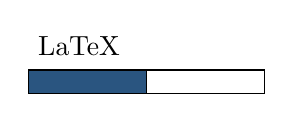
\begin{tikzpicture}
                \node [anchor=west] at (0,.6) {LaTeX};
                \draw [fill=white] (0,0) rectangle (3,.3);
                \draw [fill={rgb:red,1;green,2;blue,3}] (0,0) rectangle (1.5,.3); %50%
            \end{tikzpicture} &

            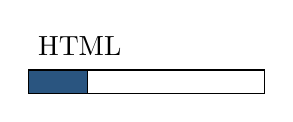
\begin{tikzpicture}
                \node [anchor=west] at (0,.6) {HTML};
                \draw [fill=white] (0,0) rectangle (3,.3);
                \draw [fill={rgb:red,1;green,2;blue,3}] (0,0) rectangle (.75,.3); %25%
            \end{tikzpicture} &

            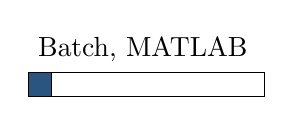
\begin{tikzpicture}
                \node [anchor=west] at (0,.6) {Batch, MATLAB};
                \draw [fill=white] (0,0) rectangle (3,.3);
                \draw [fill={rgb:red,1;green,2;blue,3}] (0,0) rectangle (.3,.3); %10%
            \end{tikzpicture} &

            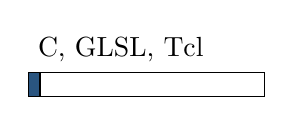
\begin{tikzpicture}
                \node [anchor=west] at (0,.6) {C, GLSL, Tcl};
                \draw [fill=white] (0,0) rectangle (3,.3);
                \draw [fill={rgb:red,1;green,2;blue,3}] (0,0) rectangle (.15,.3); %5%
            \end{tikzpicture}

            %%%%%%%%%%%%%%%%%%%%%%%%%%%%%%%%%%%%
        \end{tabular}
        \caption*{Experience using the Unity3D (C\#), Android Studio (Java) and Visual Studio (C++/C\#) IDEs.}
    \end{table}


    %%%%%%%%%%%%%%%%%%%%%%%%%%%%%%%%%%%%%%%%%%%%%%%%%%%%%%%%%%%%%%%%%%%%%%%%%%%%%%
    \begin{table}[h!]
        \centering
        \captionof*{table}{Foreign Languages}
        \begin{tabular}{llll}
            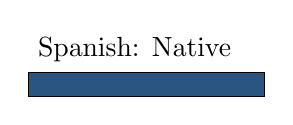
\begin{tikzpicture}
                \node [anchor=west] at (0,.6) {Spanish: Native};
                \draw [fill=white] (0,0) rectangle (3,.3);
                \draw [fill={rgb:red,1;green,2;blue,3}] (0,0) rectangle (3,.3);
            \end{tikzpicture} &

            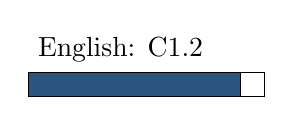
\begin{tikzpicture}
                \node [anchor=west] at (0,.6) {English: C1.2};
                \draw [fill=white] (0,0) rectangle (3,.3);
                \draw [fill={rgb:red,1;green,2;blue,3}] (0,0) rectangle (2.7,.3);
            \end{tikzpicture} &

            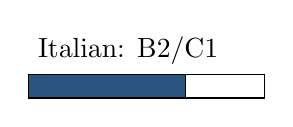
\begin{tikzpicture}
                \node [anchor=west] at (0,.6) {Italian: B2/C1};
                \draw [fill=white] (0,0) rectangle (3,.3);
                \draw [fill={rgb:red,1;green,2;blue,3}] (0,0) rectangle (2,.3);
            \end{tikzpicture} &

            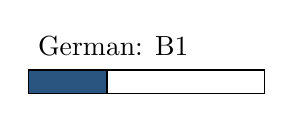
\begin{tikzpicture}
                \node [anchor=west] at (0,.6) {German: B1};
                \draw [fill=white] (0,0) rectangle (3,.3);
                \draw [fill={rgb:red,1;green,2;blue,3}] (0,0) rectangle (1,.3);
            \end{tikzpicture}
        \end{tabular}
    \end{table}


\end{rSection}
% \newpage
%--------------------------------------------------------------------
%    WORK EXPERIENCE SECTION
%--------------------------------------------------------------------

% \begin{rSection}{Experience}
%
%
% % \vspace{\baselineskip}
% %
% % \begin{rSubsection}{Delta Laboratory, MSc. Christopher Vega Sánchez}{27.07.2018–29.03.2019}{Laboratory Student-Assistant}{Cartago, Costa Rica}
% %     \item[] Manufacture of microfluidic devices with the use of photolithography and other techniques in the Investigation Project "Design and Implementation of an Impedance Spectroscopy System".
% % \end{rSubsection}
% %
% % \vspace{\baselineskip}
% %
% % \begin{rSubsection}{Orientation and Psychology Department (DOP) of TEC}{24.07.2017–09.11.2018}{Organic Chemistry Student-Tutor}{Cartago, Costa Rica}
% %     \item[] Assistance and extra lessons to students taking the Organic Chemistry course.
% % \end{rSubsection}
%
% \end{rSection}

% \\ \raggedright \small{Updated on: \today}
\vspace{\baselineskip}
\begin{flushright} \small{Updated on: \today} \end{flushright}


\end{document}
